\section{Iteracyjne metody rozwiązywania równań eliptycznych}

Będziemy korzystać z równania:

$u_{i,j} = \frac{1}{4}(u_{i+1,j} + u_{i-1,j} + u_{i,j+1} + u_{i,j-1}) - \frac{1}{4}h^2f_{i,j}$

\vspace{0.5cm}

Rozpatrzmy równanie:

\[
\begin{cases}
\vspace{0.1cm} 
\hspace{0,1cm}\frac{\delta^2 u}{\delta x^2} + \frac{\delta^2 u}{\delta y^2} = f\\
\vspace{0.1cm}
\hspace{0,1cm}u_{|\delta \Omega} = \overline{u} \\
\end{cases}
\]

, gdzie:

$(x,y) \in \Omega$

$\Omega = [a,b] \times [c,d]$

$\Omega \subset \Re^2$

\subsection{Cel ćwiczenia}

Naszym zadaniem było stworzenie algorytmu rozwiązującego następujące równania:

a) \hspace{6cm} b)

$\frac{\delta^2 u}{\delta x^2} + \frac{\delta^2 u}{\delta y^2} = 0$ \hspace{4.15cm} $\frac{\delta^2 u}{\delta x^2} + \frac{\delta^2 u}{\delta y^2} = -cos(x+y)-cos(x-y)$

, gdzie: \hspace{5.2cm} , gdzie:

warunki brzegowe: \hspace{3.5cm} warunki brzegowe:

$u(x,0) = 2lnx$ \hspace{4.15cm} $u(x,0) = cos(x)$

$u(1,y) = ln(y^2 + 1)$ \hspace{3.3cm} $u(0,y) = cos(y)$

$u(x,1) = ln(x^2 + 1)$ \hspace{3.28cm} $u(x,\frac{\pi}{2}) = 0$

$u(2,y) = ln(y^2 + 4)$ \hspace{3.3cm} $u(\pi,y) = -cos(y)$

rozwiązanie analityczne: \hspace{2.6cm} rozwiązanie analityczne:

$u(x,y) = ln(x^2 + y^2)$ \hspace{3.1cm} $u(x,y) = cos(x)\cdot cos(y)$

\vspace{0.5cm}

trzema metodami: Jacobiego, Gaussa $-$ Seidela oraz Peacemanna $-$ Rachforda.

\subsection{Metoda Jacobiego}

W metodzie tej wybieramy pierwsze arbitralne, dowolne przybliżenie rozwiązania numerycznego.

Im bliżej rozwiązania analitycznego dobrane jest przybliżenie tym mniej iteracji będziemy potrzebować w procesie iteracyjnym.

Jedna pełna iteracja polega na poprawieniu jeden raz wartości przybliżonych we wszystkich węzłach wewnętrznych siatki, aby następnie przejść do kolejnej iteracji wychodząc z tego samego węzła co poprzednio.

Dobór punktów nie ma znaczenia, ważne jest jedynie aby w kolejnych iteracjach zachować obrany porządek.

Zaletą metody Jacobiego jest nie generowanie wielkich macierzy; wadą dość wolna zbieżność.

Dowolne pierwsze przybliżenie:

$$u_{i,j}^{(n)} = \frac{1}{4}(u_{i+1,j}^{(n)} + u_{i-1,j}^{(n)} + u_{i,j+1}^{(n)} + u_{i,j-1}^{(n)}) - \frac{1}{4}h^2f_{i,j}$$

\subsection{Algorytm}

a)

//kod z jacobi1

b)

//kod z jacobi1

\subsection{Wykresy}

a)

Dla n = 5:

{\centering
	
	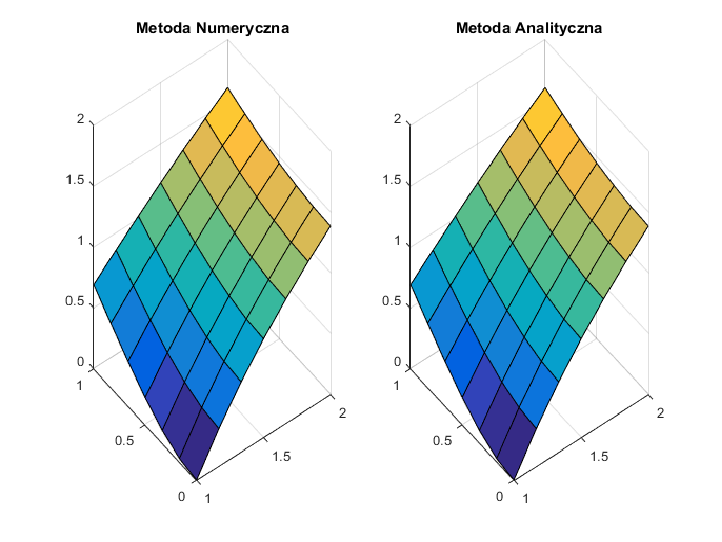
\includegraphics{Lab6/charts/jacobi/1_5.png}
	
}

Błąd metody = $8.1538e-04$

Liczba wykonanych iteracji $ = 54 $

Czas wykonywania algorytmu $ = 0.164 s$

Dla n = 15:

{\centering
	
	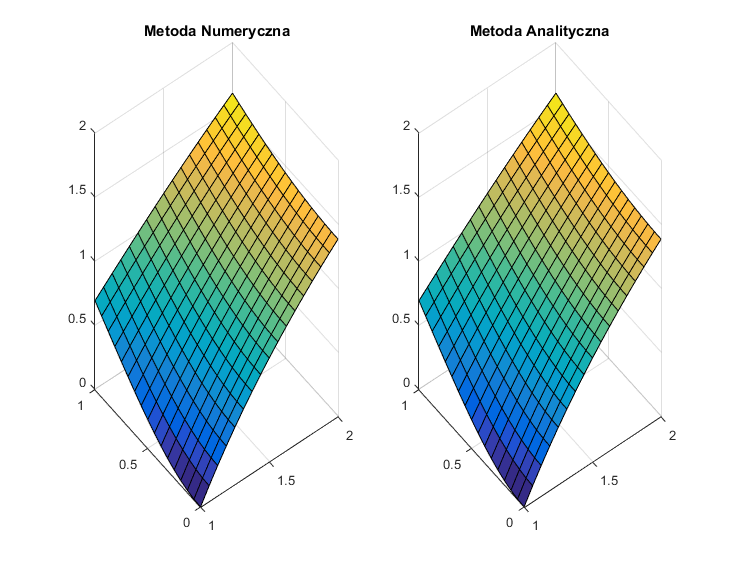
\includegraphics{Lab6/charts/jacobi/1_15.png}
	
}

Uzyskany błąd metody = $0.0051$

Liczba wykonanych iteracji $ = 292 $

Czas wykonywania algorytmu $ = 0.187 s$

\newpage

Dla n = 50:

{\centering
	
	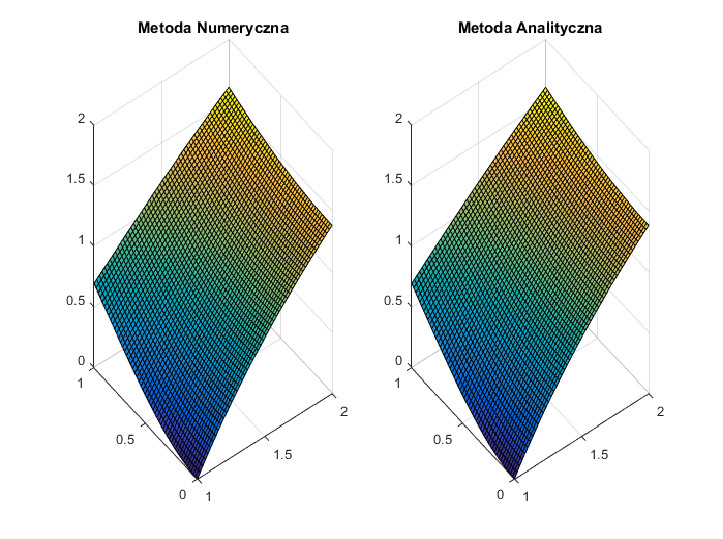
\includegraphics{Lab6/charts/jacobi/1_50.png}
	
}

Uzyskany błąd metody = $0.0526$

Liczba wykonanych iteracji $ = 1759 $

Czas wykonywania algorytmu $ = 1.523 s$

\newpage

b)

Dla n = 5:

{\centering
	
	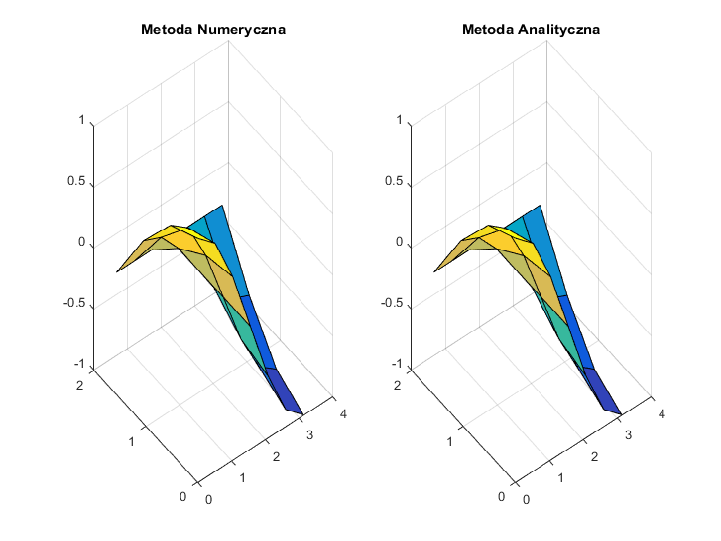
\includegraphics{Lab6/charts/jacobi/2_5.png}
	
}

Błąd metody = $0.0037$

Liczba wykonanych iteracji $ = 13 $

Czas wykonywania algorytmu $ = 0.169 s$

\newpage

Dla n = 15:

{\centering
	
	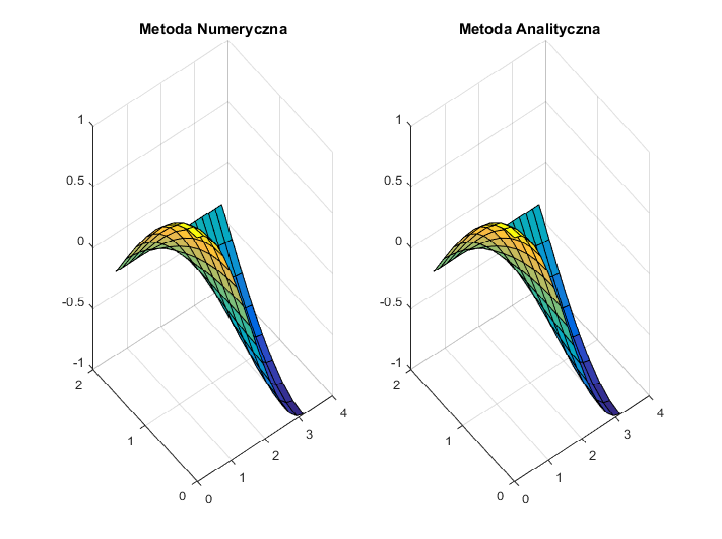
\includegraphics{Lab6/charts/jacobi/2_15.png}
	
}

Błąd metody = $6.3068e-04$

Liczba wykonanych iteracji $ = 81 $

Czas wykonywania algorytmu $ = 0.172 s$

\newpage

Dla n = 35:

{\centering
	
	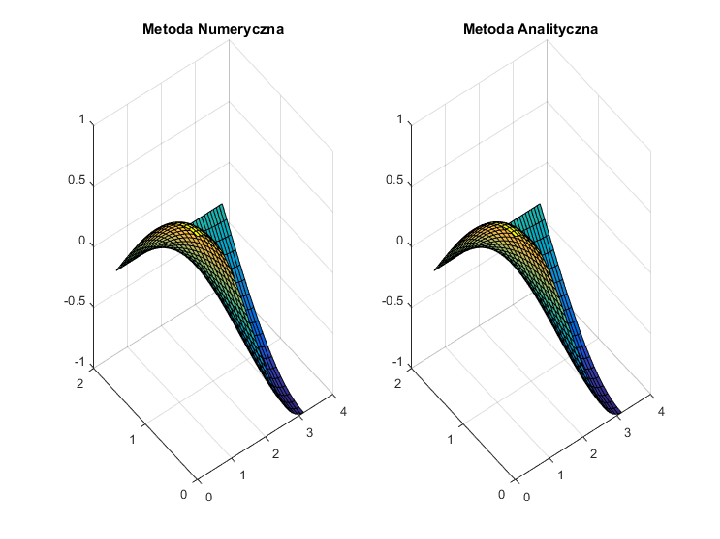
\includegraphics{Lab6/charts/jacobi/2_35.png}
	
}

Błąd metody = $    0.0063$

Liczba wykonanych iteracji $ = 308 $

Czas wykonywania algorytmu $ = 0.241s$


\subsection{Metoda Gaussa - Seidela	}

Jest to dowolona modyfikacja metody Jacobiego, a wprowadzana zmiana niemal dwukrotnie przyspiesza tempo zbieżności.

W metodzie tej wartości przybliżone rozwiązania numerycznego są poprawiane w węzłach siatki zgodnie z ustalonym przez cały proces iteraycjny porządkiem.

Dowolne pierwsze przybliżenie (poprawione):

$$u_{i,j}^{(n+1)} = \frac{1}{4}(u_{i+1,j}^{(n)} + u_{i-1,j}^{(n+1)} + u_{i,j+1}^{(n)} + u_{i,j-1}^{(n+1)}) - \frac{1}{4}h^2f_{i,j}$$

Schemat ten jest pozornie niejawny, ale w rzeczywistości uwzględnia on w kroku $n+1$ poprawkę wcześniej już obliczoną.

\subsection{Algorytm}

a)

b)

\subsection{Wykres}




